\documentclass[tikz]{standalone}
\usepackage{pgfplots}
\pgfplotsset{compat=1.15}
\usepackage{mathrsfs}
\usetikzlibrary{arrows,calc}
\usepackage{tkz-euclide}

\pagestyle{empty}

\definecolor{AngleClr}{rgb}{0,0.39215686274509803,0}
\definecolor{ShapeClr}{rgb}{0.6,0.2,0}

\begin{document}

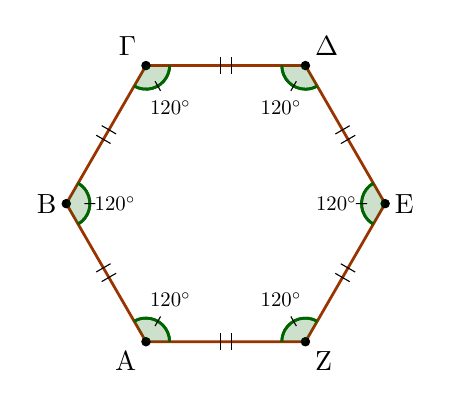
\begin{tikzpicture}[scale=.75]
\tkzSetUpLine[line width=1pt,color=black]
\tkzSetUpPoint[fill=black]

\tkzDefPoints{0/0/P0,2.7/0/P1}

\tkzDefRegPolygon[side,sides=6](P0,P1)

\tkzFillPolygon[fill=white](P1,P2,P3,P4,P5,P6)

\tkzDrawPolygon[color=ShapeClr](P1,P2,P3,P4,P5,P6)
\tkzDrawPoints[size=3](P1,P2,P3,P4,P5,P6)
\tkzLabelPoint[below left](P1){$\rm A$}
\tkzLabelPoint[below right](P2){$\rm Z$}
\tkzLabelPoint[right](P3){$\rm E$}
\tkzLabelPoint[above right](P4){$\rm \Delta$}
\tkzLabelPoint[above left](P5){$\rm \Gamma$}
\tkzLabelPoint[left](P6){$\rm B$}

\tkzFillAngles[fill=AngleClr,size=.4,fill opacity=0.2](P3,P2,P1 P2,P1,P6 P1,P6,P5 P6,P5,P4 P5,P4,P3 P4,P3,P2)
\tkzMarkAngles[line width=1pt,size=.4,color=AngleClr](P3,P2,P1 P2,P1,P6 P1,P6,P5 P6,P5,P4 P5,P4,P3 P4,P3,P2)
\tkzMarkAngles[mark=|,mksize=2,line width=1pt,size=.4,color=AngleClr](P3,P2,P1 P2,P1,P6 P1,P6,P5 P6,P5,P4 P5,P4,P3 P4,P3,P2)

\tkzMarkSegments[mark=||,size=3](P1,P2 P2,P3 P3,P4 P4,P5 P5,P6 P6,P1)

\tkzLabelAngles[scale=0.75,pos=1.1](P3,P2,P1 P2,P1,P6 P1,P6,P5 P6,P5,P4 P5,P4,P3 P4,P3,P2){$120^\circ$}

\end{tikzpicture}

\end{document}
